\section{ニコ書を支える快楽天}

\subsection{目標の共有}

プロジェクトを成功に導くにはチーム共通の目標が必要です。
ニコ書チームが当初に掲げた最終目標は快楽天を配信することでした。

\subsection{ソーシャルリーディング}

ソーシャルリーディングというわけのわからない単語が電子書籍業界には付きまとってきます。
ホント意味わかんないですよね。 読書体験を共有?とかそもそも友達いねーし。

でもそんな俺でも過去に読書体験を共有したことがありました。
それは完全に実益に基づいたフラット関係、 敬意と感謝に溢れた平和な世界、
すなわちエロ本の回し読みです。
エロの前でのみ、人類は平等になり、最適化され、団結できるのです。

我々は最強のエロ本プラットフォームを作る決意をしました。

\subsection{ホットモック}

システムの設計をはじめる前に、
必要な機能を絞り出したり、使用感のイメージを確認するために、
単純なサンプルを作って検討することがあります。

これを \textbf{モック} と言い、紙にUIを書いてみたり、
htmlだけをとりあえず実装してみたり、
ハードウェアの場合はガワとボタンだけ作ったりします。

特に実際に動作するモックを \textbf{ホットモック} と言い、
携帯ショップに置かれている実際に動く端末サンプルなどがこれに当たります。

もちろん、これから作る最強のエロ本プラットフォームも、
モックを使ってイメージを育てる必要があります。

ホットモックとして使ったんはもちろん本物の快楽天。
快楽天を回し読みし、抜いた場所にシールを貼っていきました。
最初はGoogle+の+1シールを、後に+1とFacebookのイイねを合わせたオリジナルのエロいねシールを使いました。

\begin{figure}[H]
  \centering
  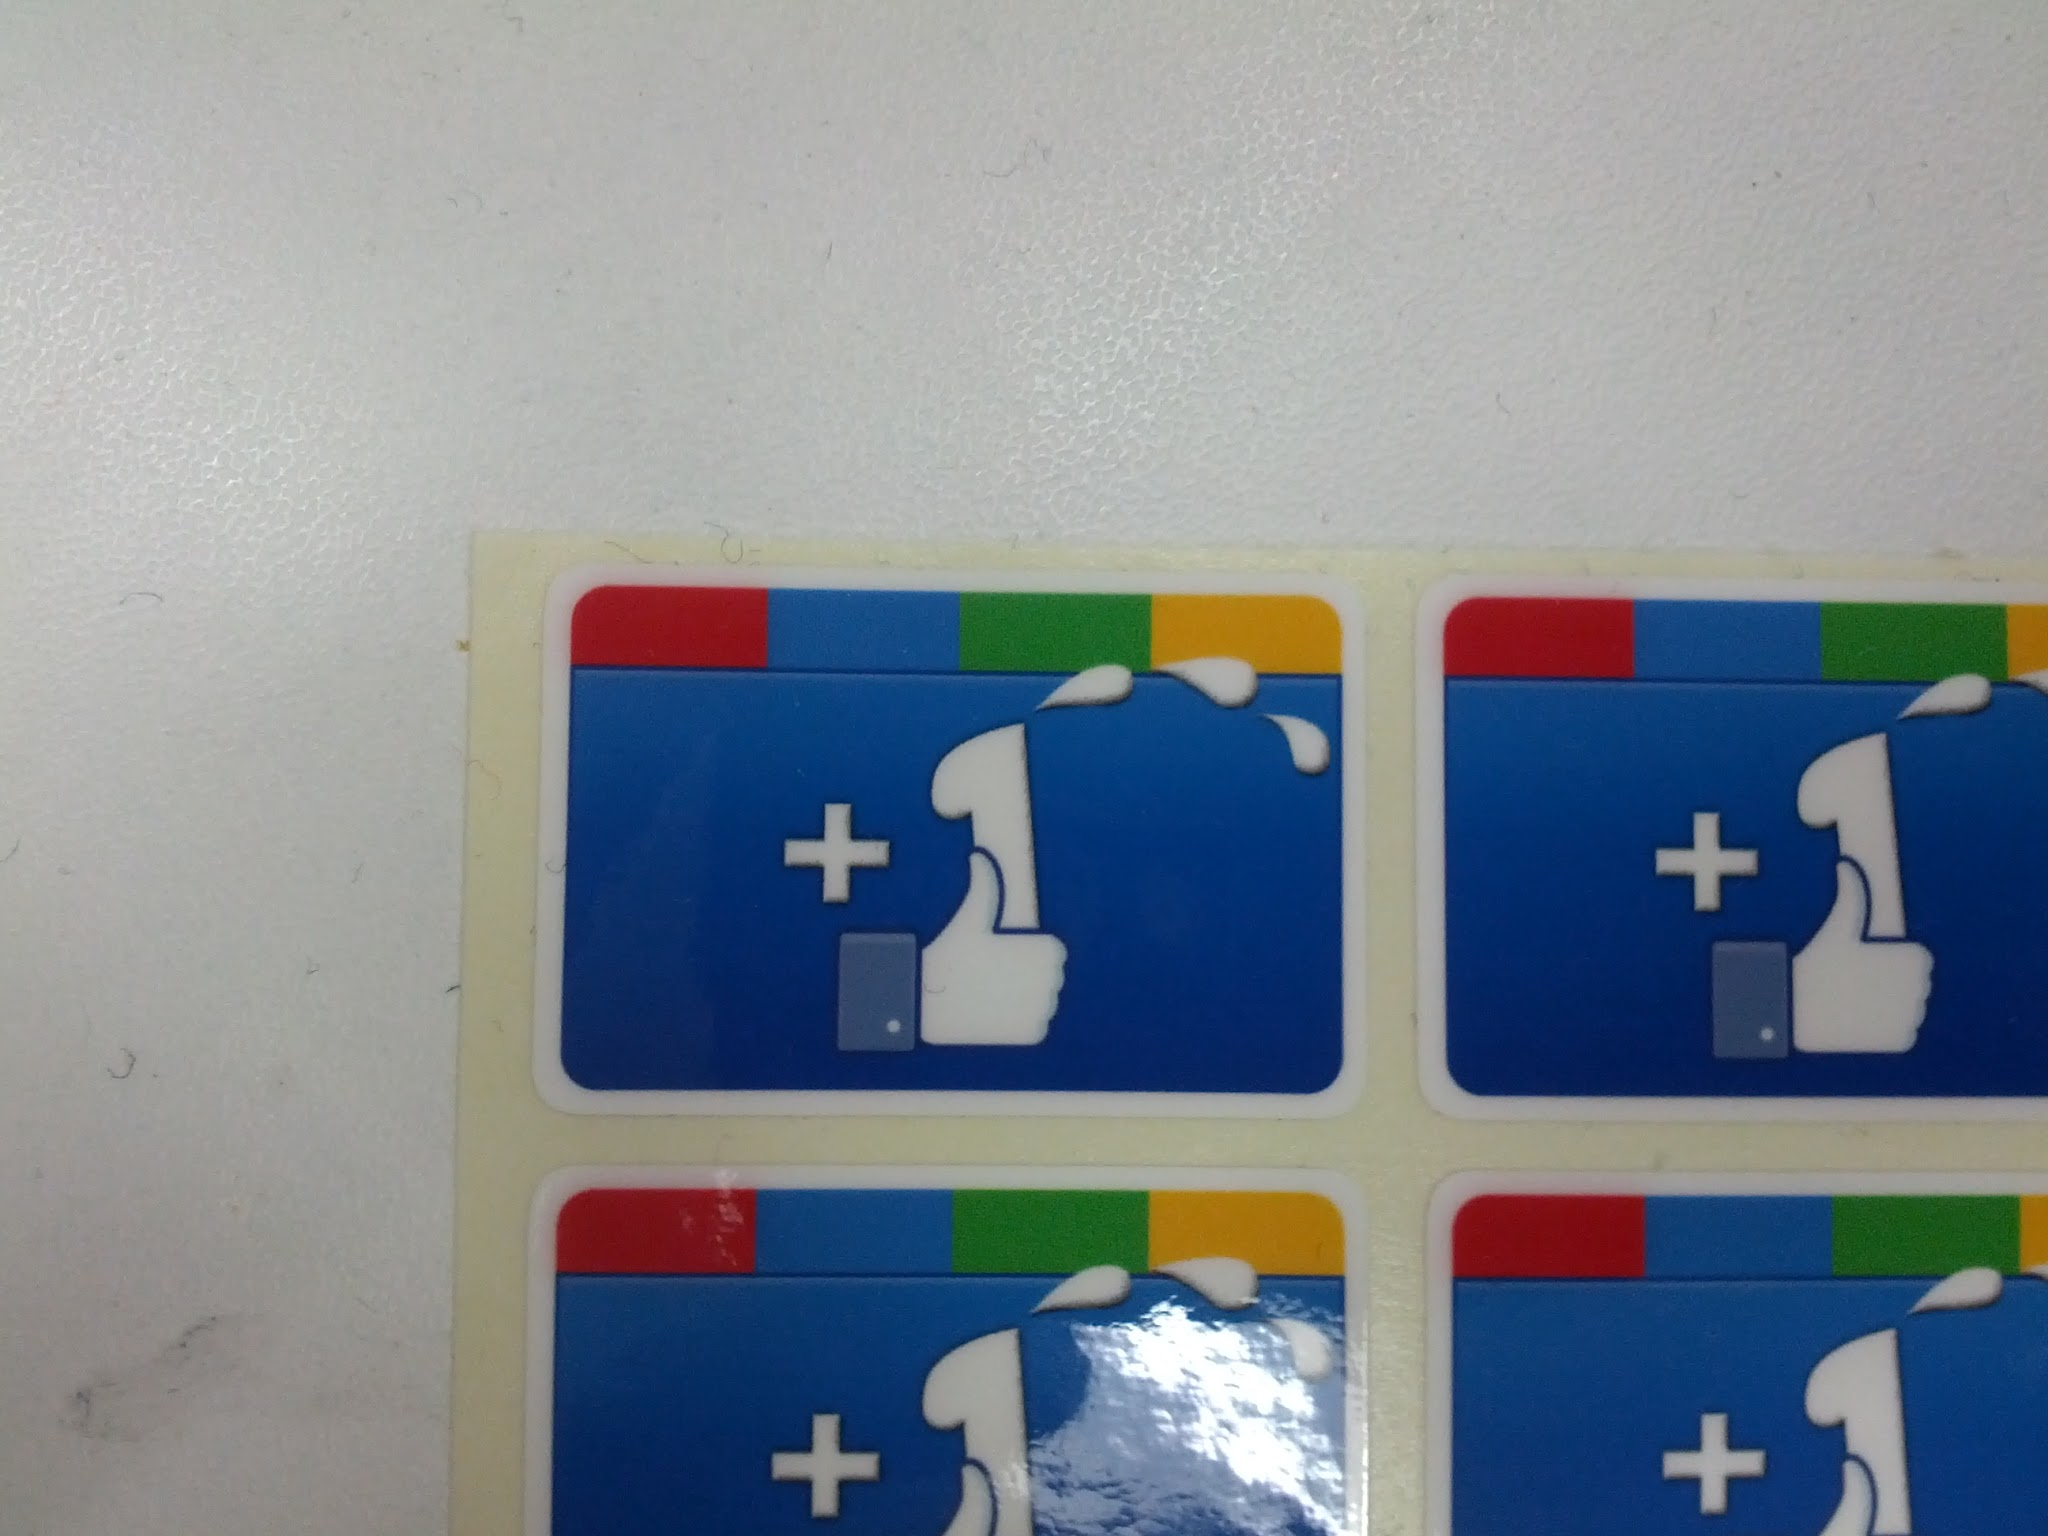
\includegraphics[width=0.5\textwidth]{../images/eroine.jpg}
  \caption{エロいねシール}
\end{figure}

\subsection{実験結果}

数ヶ月実験を続けた結果、
抜いたポイントの類似度を元にしたリコメンドシステムのモデルや、
エロいコマを軸にしたコミュニケーションの発生など、たくさんの恥見が溜まりました。

これを総称して「ソーシャルオナニー」略して「ソニー」と呼び、
この機能を実装したプレイヤーを「ソニーリーダー」と呼ぶことに決めました。

\begin{figure}[H]
  \centering
  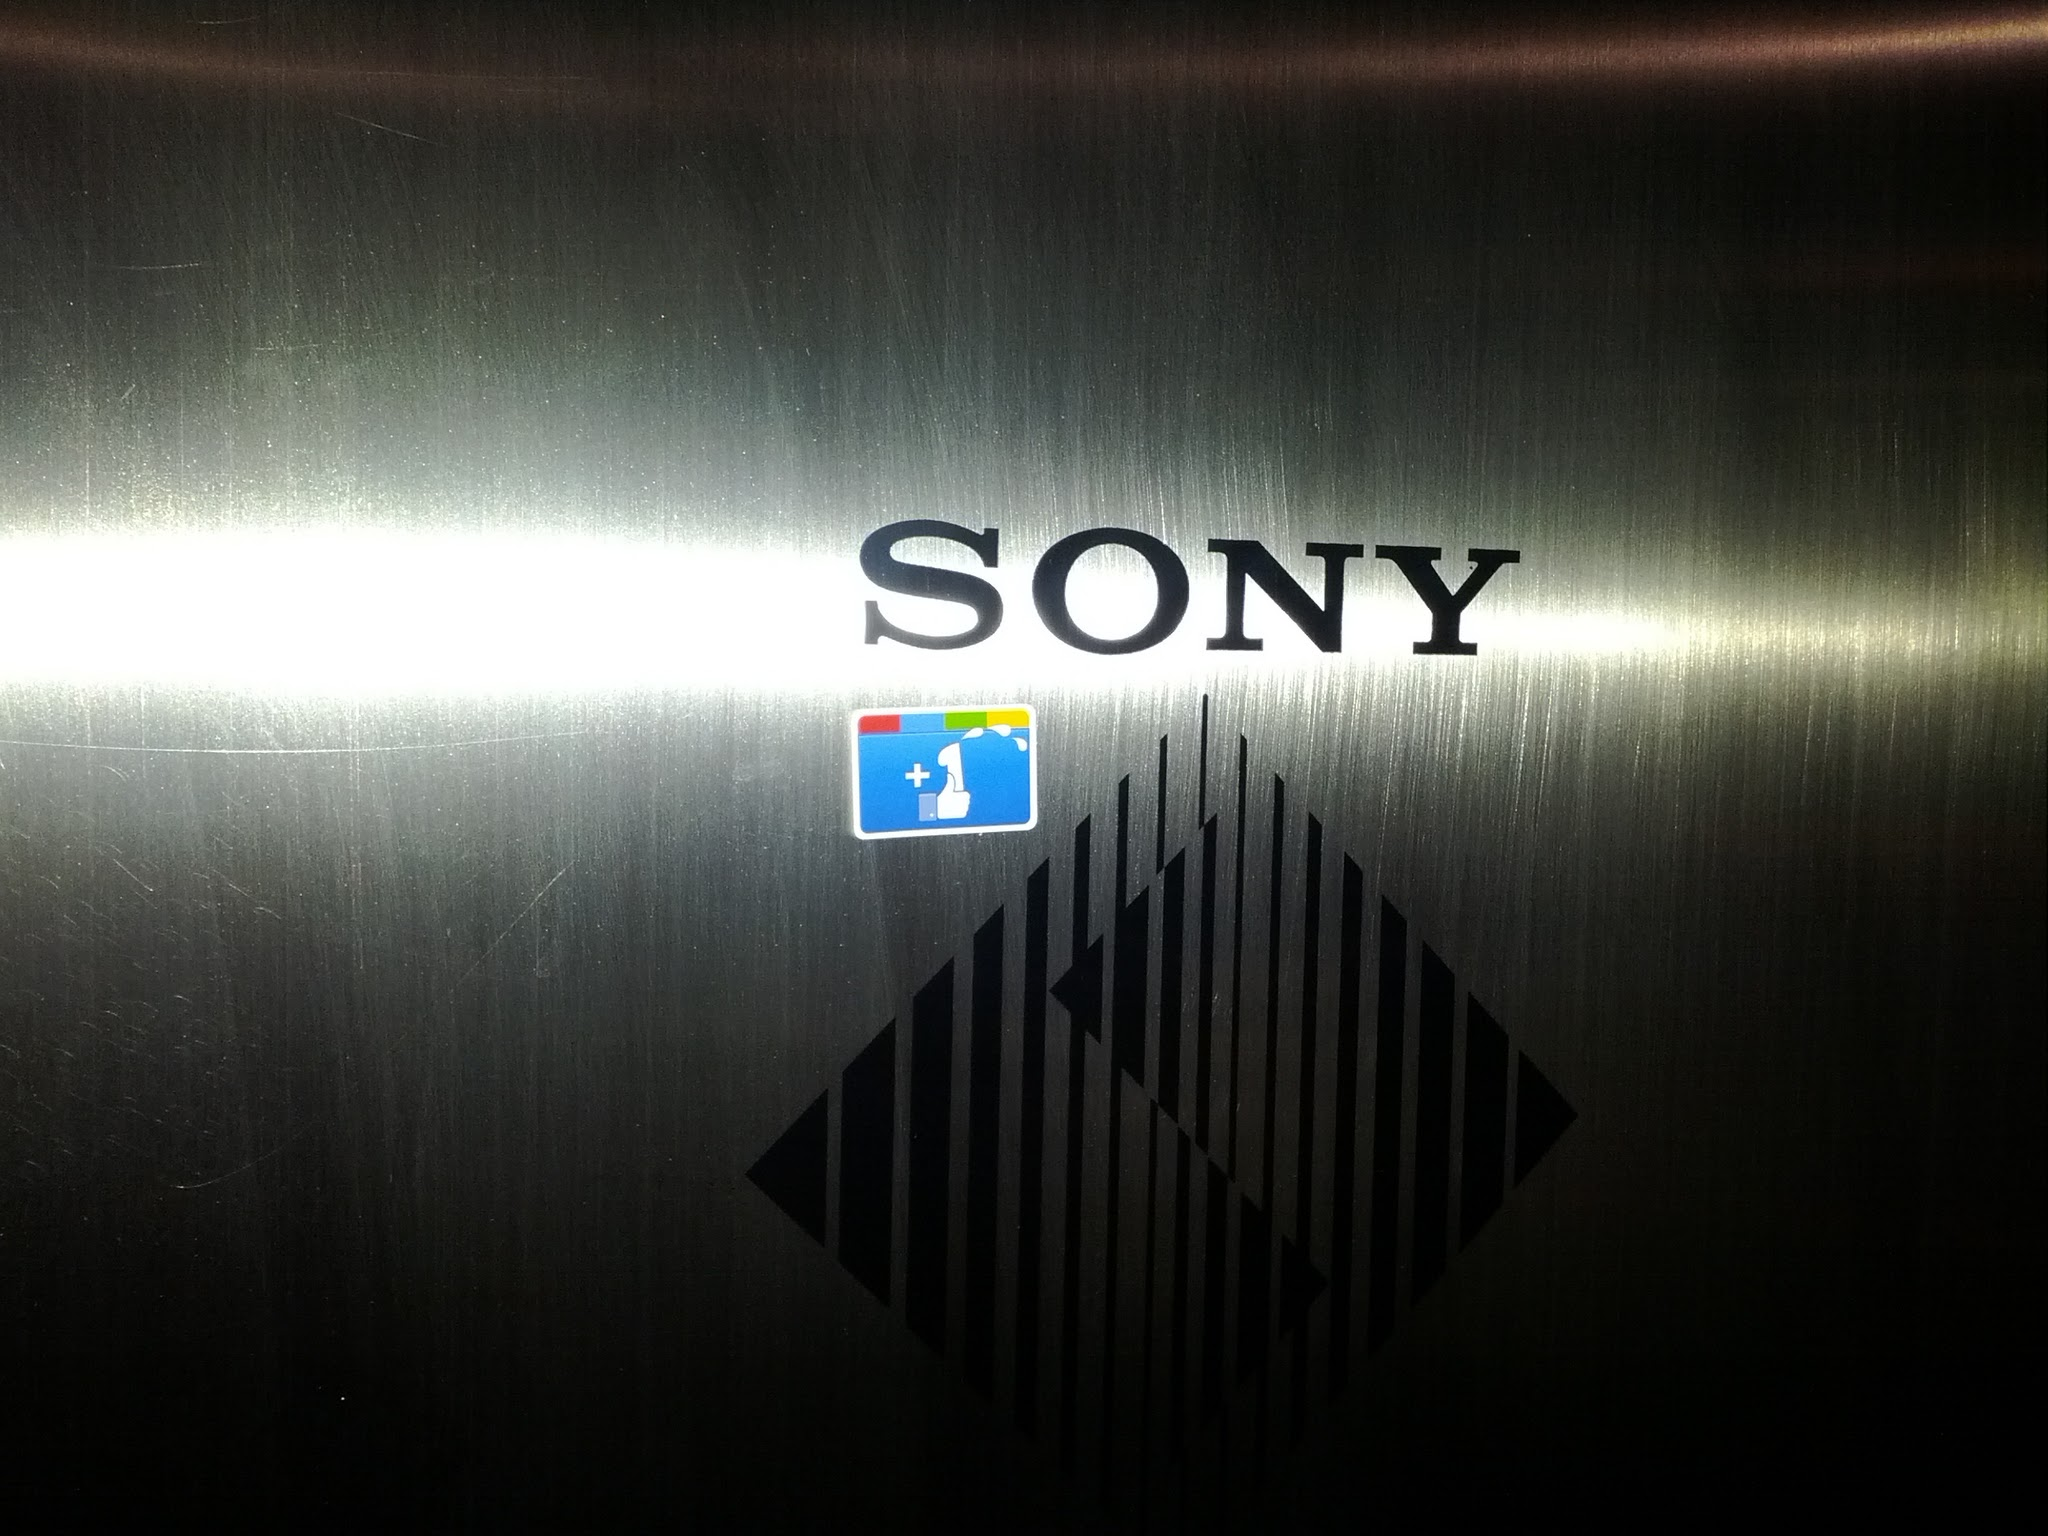
\includegraphics[width=0.5\textwidth]{../images/sony_reader.jpg}
  \caption{イッツアソニー}
\end{figure}

ソーシャルオナニーのイメージはほぼ完成し、
あとは快楽天の配信開始と、ソニーリーダーの実装開始を待つばかりとなりましたが、
静画のボスの「 \textbf{快楽天よりLOが読みたい}
」の鶴の一言により、未だにプロジェクトはペンディングとなっています。
